\autsection{Microscope}{Fruzsina Bacso}

\subsection{The microscopes main role in the mission}

A microscopic imager and spectrometer could play an essential role in our mission which is to find life on the Jovian satellite Europa. It may provide key biological and texture information as a supplementary to the other proposed instruments such as the HPLC, Raman spectroscopy and the Lab-on-a-chip (LOC) systems which are dealing with bio organic chemistry analysis as well. It has a main focus on the light element analysis so it could also form a strong complement to the XRF analyzer which deals with the heavy element detection.

The proposal of the microscope was developed on the basis of the CIVA (Comet Infrared and Visible Analyser) instrument which was designed for the Rosetta Lander Philae. CIVA-M is a combination of two miniaturised and compact microscopes, one operating in the visible light region and one in the infrared region, which embodies an IR hyperspectral imaging spectrometer.
\cite{Bibring2007}

The microscope could characterize the texture, the albedo, and the molecular composition of the samples which are collected by a filtration system. This non-destructive analysis would be the first in line to be carried out on the water samples.

It could also give information on the particles size, its shape and colour. In addition to this, imaging before and after UV illumination could provide us valuable knowledge upon the flourescence phenomenon emitted by prebiotic or biotic organic molecules and not to mention that we could as well gain information on the motility of the examined molecules if there were any.
\cite{Gowen2011725}

\subsection{Microscopic imaging development in other missions}
Emerging the visible microscopic imaging with the near-infrared spectrometry is proven to be the most effective way to study planetary materials. While the images are providing the physical characteristics of the examined object, the spectrometry gives access to the composition of the materials.

The development of these in-situ, multifunctional payoads 
started with the CIVA-M/I NIR hyper-spectral microscope which was embedded onboard Philae, the Rosetta lander that landed on comet 67P/Churyumov–Gerasimenko in 2014.

The progress in the design of a hyper-spectral imaging came with the new generation of the microscope, MicrOmega in the scope of the ESA/ExoMars rover.
\cite{Pilorget201342}

\subsubsection{Characteristics of CIVA-M microscope \cite{Bibring2007}}


The CIVA instrument is built in Philae, the Rosetta space probes lander module which was developed by the European Space Agency and launched on 2 March 2004. After a decade, on 6 August 2014 the lander reached the 67P/Churyumov–Gerasimenko comet. The Philae lander is contiually returning data from the comets surface on the purpose of studying the comets surface.
\cite{wiki:Rosetta}


Infrared reflectance spectroscopy is a convenient and powerful technique which helps to evaluate the molecular and mineralogical composition of the comet.

The CIVA-M microscope has a spectral range of 1 to 4 $\mu m$ which allows the scientists to probe and explore the rich variety of chemical composition comprising the grains in the comet samples.
Molecules for instance $H_2O$, $NH_3$, $NH_4SH_3$, $H_2CO$, $CH_3OH$, $CH_3CN$, $HCN$, $H_2S$, $CO$, $CO_2$ and $CH_4$ can be identified within this spectral range.

As it was mentioned before, CIVA-M embodies two microscopes, a visible light microscope CIVA-M/V and a near-infrared hyperspectral imager called CIVA-M/I. Both instruments are mounted on the balcony of  the Philae lander next to the sample distribution system (SD2).

The sample collector and process system analyses the comet material (from the distance of 13 mm) gathered in containers (“Mid Temperature
Ovens”) which are mounted on a rotating carousel. The containers are isolated from the microscope lens with a saphire window transparent in both visible and near-infrared.

CIVA-M/V images the samples onto a 1024 × 1024 CCD detector with a spatial sampling of 7 $\mu m$ and a depth of focus up to 0.1 mm. The illumination sources are three LEDS working at 525 nm (green/blue), 640 nm (red) and 880 nm (near IR). The mass and size of the visible light microscope is 276 g and 70 × 50 × 94 $m^3$. 

Regarding the IR spectral images, the detection is done by a 128×128 photovoltaic HgCdTe array (spatial sampling 40 $\mu m$) operating at temperatures 120 to 140 K. The appropriate temperature is provided by a passive radiator cooling. 

The microscope is using a white light source coupled in front of a grating monochromator which provides the chosen wavelength. The monochromatic light illuminates and scans the sample over the spectral range 1 and 4 $\mu m$, with steps of 3 nm. About 750 images are taken at a different wavelength which is stored in a 3-dimensional "image-cube" which will be described in details in the following section. The imaging process takes approximately 20 minutes and gives a spectra with SNR over 100, assuming IR albedos of 0.05. The mass and size of CIVA-M/I are: 455 g and 80 × 50 × 120 $m^3$.
The following table summarizes the specifics of the CIVA-M microscope. 
\ref{fig:CIVAM_specs}

\begin{figure}[htb]
  \centering
  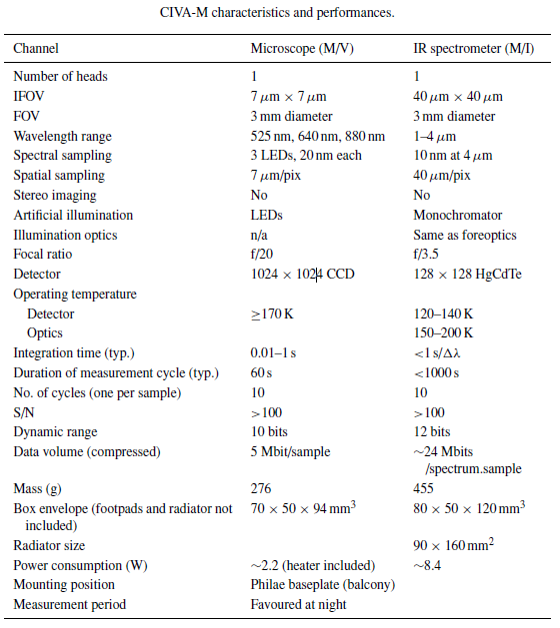
\includegraphics[scale=0.7]{figures/BFfig/CIVAM_specs}
  \caption{CIVA-M specifications and performance}
  \label{fig:CIVAM_specs}
\end{figure}



\subsubsection{Design of the MicrOmega/IR instrument} 

The MicrOmega/IR instrument was developed at IAS (Institut d'Astrophysique Spatiale, Orsay, France), however it inherited many things from the development used in the CIVA/M. It is a part of the payload of ESA/ExoMars mission. 

The main objective of the microscope is to analyze the samples collected on Mars in a non-destructive way at the scale of grain size.
\ref{fig:Block_diagram}

\begin{figure}[htb]
  \centering
  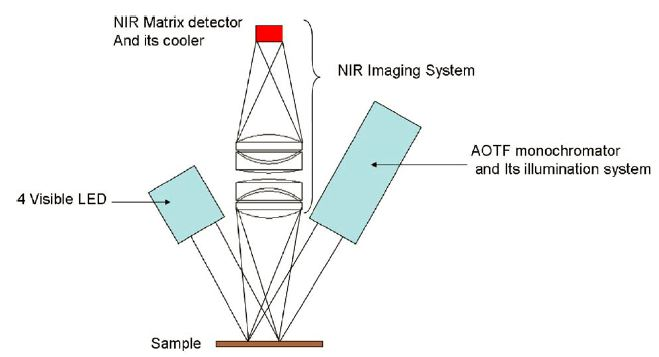
\includegraphics[scale=0.8]{figures/BFfig/Block_diagram}
  \caption{The block diagram of the MicrOmega/IR}
  \label{fig:Block_diagram}
\end{figure}

The instrument is working in the spectral range of 0.9–2.6 mm and in 4 wavelengths in the visible region with LED light source.
\cite{Leroi20091068}

It will obtain in situ reflectance spectra of the collected samples with a spatial sampling of 20 mm per pixel. The monochromatic light source illuminates the sample (5 mm sized) in 320 spectral channels.
\ref{fig:Specs_for_MicrOmega}

\begin{figure}[htb]
  \centering
  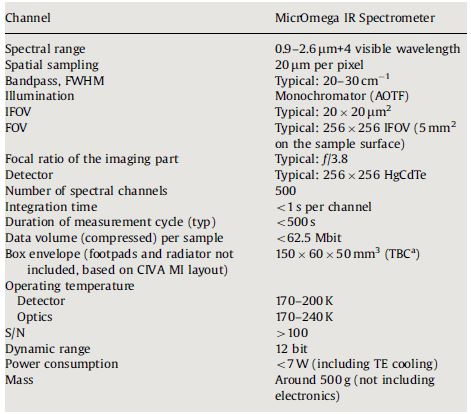
\includegraphics[width=.48\textwidth]{figures/BFfig/Specs_for_MicrOmega}
  \caption{The technical specification table of MicrOmega/IR}
  \label{fig:Specs_for_MicrOmega}
\end{figure}

The microscope will take an image on each wavelength which will be detected with a matrix detector. As a result the information will be saved on a 3-dimensional  'Image Cube'. The cubes spatial coordinates are [X,Y] whereas the third dimension is the wavelength. For each pixel with this method the full spectrum of the inspected samples can be found, including all the 320 spectral elements, as shown in Figure \ref{fig:Image_cube}.

\begin{figure}[htb]
  \centering
  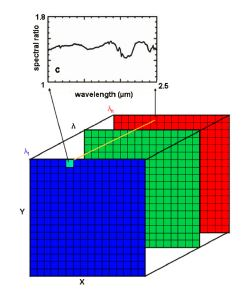
\includegraphics[width=.48\textwidth]{figures/BFfig/Image_cube}
  \caption{The image cube is composed of 2 spatial dimensions (X,Y) and the wavelength}
  \label{fig:Image_cube}
\end{figure}

\paragraph{The light sources and the acousto-optic tunable filter}

For the MicrOmega microscope a commercial tungsten filament lamp was chosen (manufactured by Gilway with the reference T1 1088-9A). The bulb has a wide spectrum from visible up to 4 mm and provides strong illumination with a low consumption (0.5 W). The illumination system was also qualified for its lifetime, as well for its operating in vacuum and at low temperatures.

The acousto-optic tunable filter has the same role as a monochromator. It operates in a very simple and elegant way. The acoustic wave attains a tension in a crystal and as a consequence it changes its optical properties. Due to this interaction between the light and the acoustic wave, the light gets diffracted in line with the frequency of the acoustic wave.

The acoustic waves are generated by piezoelectric transducers. These transducers are excited by radio-frequency which leads to acoustic field in the crystal. By tuning the RF frequency the adequate wavelength is chosen, and correspondingly the sample is illuminated with the monochromatic light. This process is repeated to cover the entire spectral range.

One significant and considerable advantage of the acousto-optic tunable filter is that it is compact and has no moving part. Therefore during the scanning procedure the sample, as well as the illuminating light beam is mechanically stable.

\paragraph{The NIR imaging matrix detector}
Regarding the detection of the illuminated samples, a 256 x 256 pixels HgCdTe low dark current matrix detector is used. The spectral range as it was mentioned previously is 0.5-2.6 mm with a cut off wavelength of 2.55 mm.
A thermo electric cooler is needed for cooling down the detector to its most favourable operational temperature which is around 190 K. The specification for the matrix detector are summarized in the following table.
\ref{fig:Specs_for_NIR_detector_MicrOmega}

\begin{figure}[htb]
  \centering
  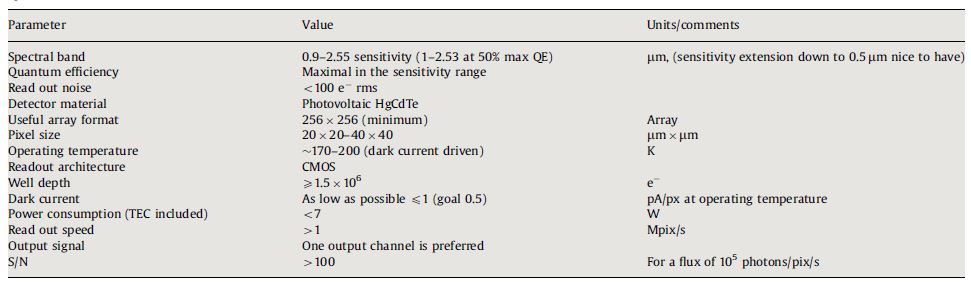
\includegraphics[scale=0.6]{figures/BFfig/Specs_for_NIR_detector_MicrOmega}
  \caption{Specifications for the near-infrared detector}
  \label{fig:Specs_for_NIR_detector_MicrOmega}
\end{figure}


\subsection{Implementation}
In the matter of designing a microscope for our specific needs first of all we had to look into the theory and search for other implementations to see what we could we utilize from the other missions. In the previous section two very similar but different designs were presented. In this section we are making an attempt for a design plan which we could use in our mission to Europa.

\subsubsection{Notch filtering}

One of the main difference between our mission and the previous two is the material in which we are searching for life. On a comet one could search after and examine for example minerals and ices. Compared to Europa where we are presuming only ice and water.

As a matter of fact if we would like to see something from our measurements we need a filter embedded in front of the sensor to filter out the wavelengths resulted from $H_2O$. As it is demonstrated in the picture below, the water has a low absorption coefficient in the visible light spectra, however it is increasing towards the infrared region. Consequently between the frequency range of 3000 and 4000 $cm^{-1}$ we could see no results because of the high $H_2O$ response.
\ref{fig:Absorption_coeff_water}

\begin{figure}[htb]
  \centering
  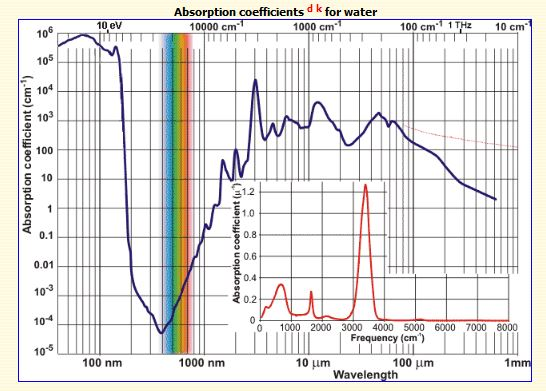
\includegraphics[scale=0.7]{figures/BFfig/Absorption_coeff_water}
  \caption{The visible and UV spectra of water}
  \label{fig:Absorption_coeff_water}
\end{figure}

Installing a notch filter into the optical path (also commonly referred to as band-stop filters) could attenuate the light within the 3000 and 4000 $cm^{-1}$ range and as a result we could obtain a better signal-to-noise ratio.

On the market Thorlabs has a wide range of optical notch filters however currently they only offer filters with central stop-band wavelengths of 405, 488, 514, 533, 561, 594, 633, 658, 785, 808, 980, or 1064 nm which is not good for our application.
\cite{filters}

As a consequency it might be doable if we could use a low-pass filter with cut-off frequency at 3000 $cm^{-1}$ and a high-pass filter with cut-on wavelength of 4000 $cm^{-1}$ placed after each other. Since the current market does not offer filters in this region this may require further market- research.

\subsubsection{Near-infrared and visible light source}

Since the MicrOmega microscope had a feasible and cheap solution to the IR light source, we decided to use it in our mission, together with the acousto-optic tunable filter. 

As it was described before, the commercial tungsten filament lamp (T1 1088-9A Gilway) is a great choice because it has a wide spectrum and provides strong illumination with a low consumption. It is also qualified for space environment which is the most important.
\ref{fig:IR_light_source}
\ref{fig:MicrOmegaVISandIR}

With regard to the visible light LED sources, further investigation is needed since choosing 12 commercial different wavelengths LEDs  could be an option for us but qualification for space application is needed just like it had been performed with the IR source.
\ref{fig:MicrOmegaVIS}
\ref{fig:MicrOmegaVISandIR}

\begin{figure}[htb]
  \centering
  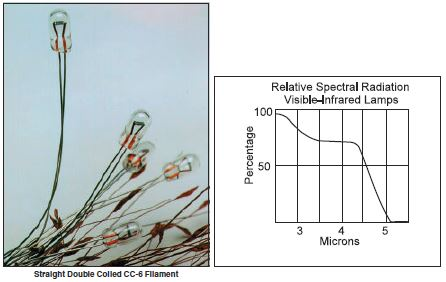
\includegraphics[scale=0.6]{figures/BFfig/IR_light_source}
  \caption{Infrared light source \cite{halogenlamp}}
  \label{fig:IR_light_source}
\end{figure}


\begin{figure}[htb]
  \centering
  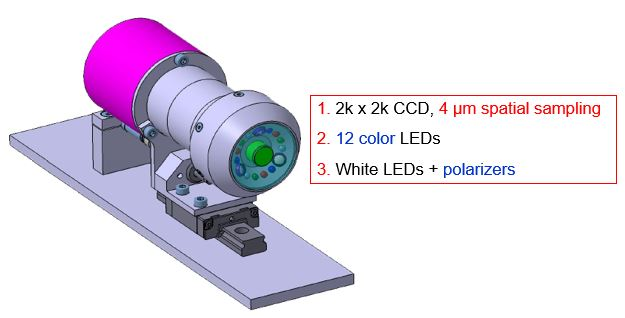
\includegraphics[scale=0.6]{figures/BFfig/MicrOmegaVIS}
  \caption{The visible light source unit \cite{Bibring_MicrOmega}}
  \label{fig:MicrOmegaVIS}
\end{figure}

\begin{figure}[htb]
  \centering
  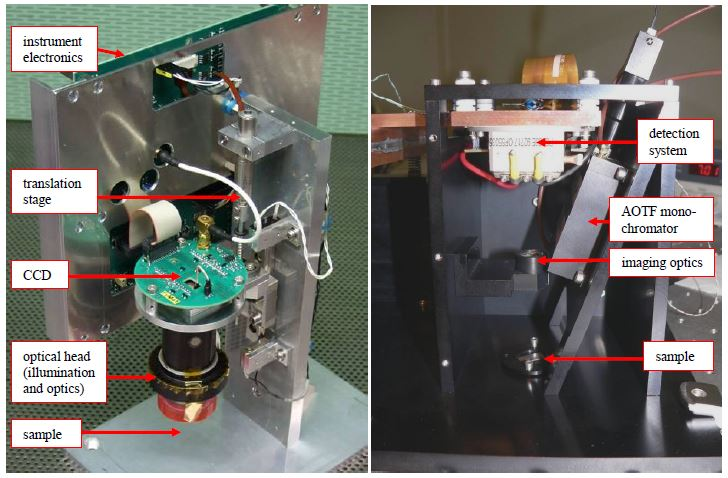
\includegraphics[scale=0.6]{figures/BFfig/MicrOmegaVISandIR}
  \caption{The MicrOmega visible and infrared microscope \cite{Mars_Micromega}}
  \label{fig:MicrOmegaVISandIR}
\end{figure}


\subsubsection{The acousto-optic tunable filter (AOTF)}
The same way as the light source, the acousto-optic tunable filter could be used as our monochromator in the mission. In the MicrOmega/IR section it was described adequately. On the following picture the acousto-optic tunable filter can be seen during operation.
\ref{fig:AOTF_operation}


\begin{figure}[htb]
  \centering
  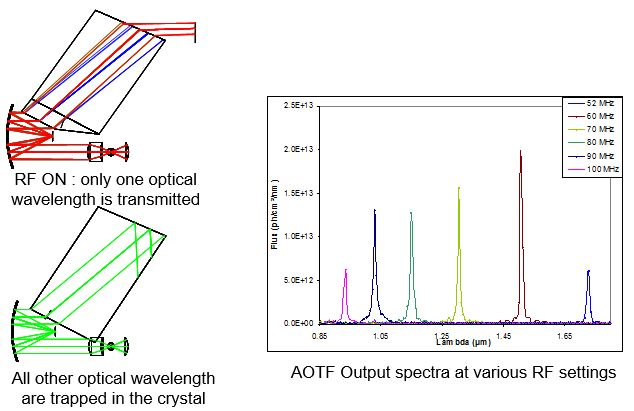
\includegraphics[scale=0.5]{figures/BFfig/AOTF_operation}
  \caption{The acousto-optic tunable filter in operation}
  \label{fig:AOTF_operation}
\end{figure}

\subsubsection{The light detectors}

\paragraph{The CCD for visible light detection}

For visible light imaging we could use the KAF-16801 high performance area CCD (charge-coupled device) image sensor with 4096H x 4096V photo active pixels. The table below shows its specifications operating in 298 K temperature which is suitable for us.
\ref{fig:CCD_sensor}

\begin{figure}[htb]
  \centering
  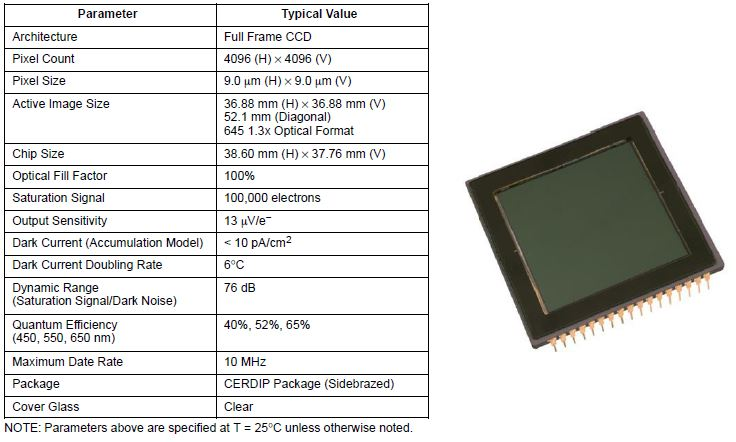
\includegraphics[scale=0.6]{figures/BFfig/CCD_sensor}
  \caption{The proposed CCD sensor \cite{CCDsensor}}
  \label{fig:CCD_sensor}
\end{figure}


\paragraph{The microbolometer for near-infrared measurements}
Microbolometers are a sophisticated alternative to longwave infrared photon detectors since they are detecting the radiant heat rather than photons. Due to the fact that they do not require cooling reduces their complexity as well as their size and cost. Improvements in the production technology made it possible to increase their sensitivity and array size which makes them more practical and affordable.

For the near-infrared detection a Rockwell manufactured, VOx bolometer with 48 x 48 pixel size and 300 K operating temperature would be the best option, however this may require a light source in the far infra spectrum (in the 8-14 $\mu m$ range). Our chosen tungsten filament lamp does not provide this wide scale of spectrum so further investigation should be made whether we should change the light source or choose a different type of microbolometer which would probably need a cooling unit. 
\ref{fig:Microbolometer}

\begin{figure}[htb]
  \centering
  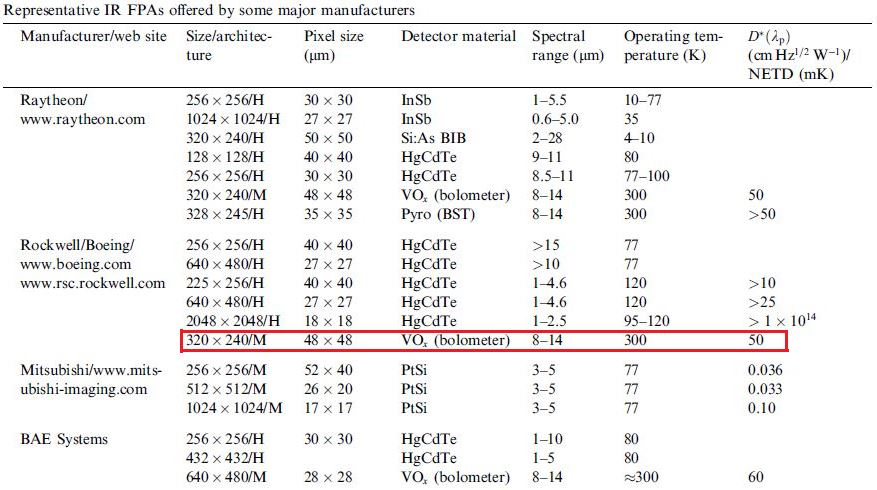
\includegraphics[scale=0.6]{figures/BFfig/Microbolometer}
  \caption{The microbolometer specification \cite{Rogalski2002187}}
  \label{fig:Microbolometer}
\end{figure}
